% This is samplepaper.tex, a sample chapter demonstrating the
% LLNCS macro package for Springer Computer Science proceedings;
% Version 2.20 of 2017/10/04
%
\documentclass[runningheads]{llncs}
%
\usepackage{graphicx}
% Used for displaying a sample figure. If possible, figure files should
% be included in EPS format.
%
% If you use the hyperref package, please uncomment the following line
% to display URLs in blue roman font according to Springer's eBook style:
% \renewcommand\UrlFont{\color{blue}\rmfamily}

\begin{document}
%
\title{Técnicas y Herramientas Modernas}
%
%\titlerunning{Abbreviated paper title}
% If the paper title is too long for the running head, you can set
% an abbreviated paper title here
%
\author{Muscianisi,M.;  Frias,F.;  Clement,M.;  Ibañez, S.;  Campati,B.;  Cuevas,J.}
%

% First names are abbreviated in the running head.
% If there are more than two authors, 'et al.' is used.
%
\institute{Universidad Nacional de Cuyo}


%
\maketitle              % typeset the header of the contribution
%

%
%
\section{Gases efecto invernadero}
\subsection{Algunos gases y de donde provienen}
La agricultura y la ganadería son grandes responsables de la emisión de gases efecto invernadero, ésta última es una gran fuente de emisión de gas metano(un gas mas potente que el CO2) y amoniaco, además de que consume gran cantidad de agua.
Algunos autores sostienen que la agricultura y las infraestucturas hidricas son grandes responsables de la emisión de gases efecto invernadero y que es muy importante ver que estos estan interconectados entre si.(Dustin Mulvaney,2020,pag 218)
\begin{figure}
\includegraphics[width=0.7\textwidth]{ganaderia1.jpg}
\end{figure}









\subsubsection{Algunas soluciones al respecto}  En el libro Sustainable energy transitions de Dustin Mulvaney se sostiene que algunas de las soluciones para reducir la emisión de gases efecto invernadero son la utilización de energías renovables, incluso también el uso de tierras "marrones" (contaminadas por la sal) en desuso para su transformación en granjas solares,etc.
A su vez Dustin Mulvaney también afirma que se crearon sistemas para solucionar los problemas entre alimentos, energía y agua llamados FEW, que tienen varias aplicaciones y grandes alcances(2020,pag 219)
 

\subsection{Transición energetica}
Dustin Mulvaney expresa en su libro Sustainable energy transitions que para lograr una transición energetica se necesita un uso responsable y sostenible de la energía e introducir formas diferentes a las convencionales para su producción, basadas en energías renovables.
\begin{figure}
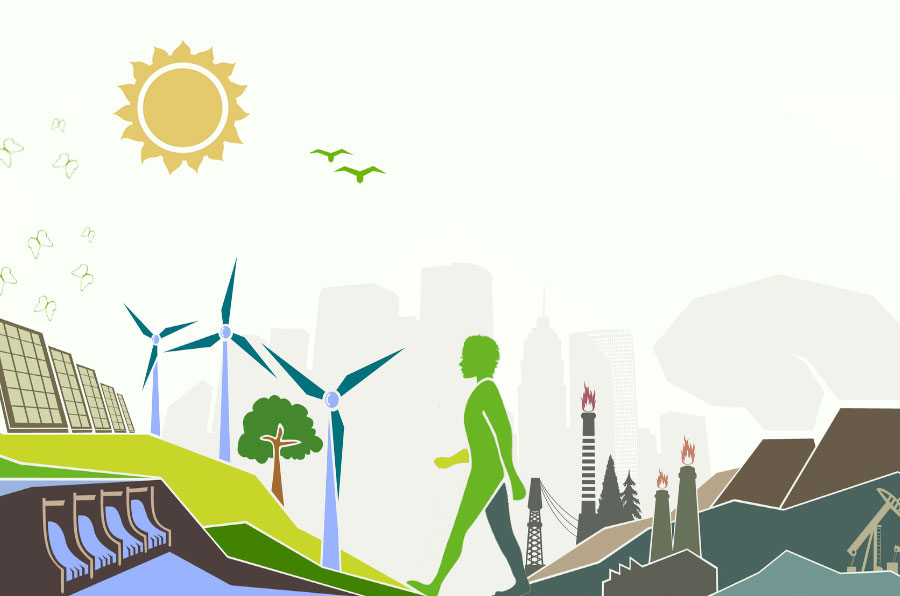
\includegraphics[width=0.7\textwidth]{transicion-energetica-1.jpg}
\end{figure}

\paragraph{Conclusión}
El paso hacia la descarbonización es largo, se necesitan varios factores para lograrlo, desde politicas públicas que ayuden a reducir el mal uso de las energias, hasta el desarrollo de nuevas teconologías.

El gran problema que hay para lograr una descabornización eficiente es en gran parte económico, cada uno persiguer sus propios intereses y más aún despues de un año muy complicado como lo fue el 2020, donde la economía cayó considerablemente. Apuntar hacia nuevos objetivos mas ecológicos no pareciera ser una buena idea al momento de querer repuntar si no más bien seguir por el camino de los combustibles fósiles. 
  
 
 También la sociedad tendrá que cambiar y tener en cuenta que algunos se verán perjudicados por estas transiciones.






%
% the environments 'definition', 'lemma', 'proposition', 'corollary',
% 'remark', and 'example' are defined in the LLNCS documentclass as well.
%


%
% ---- Bibliography ----
%
% BibTeX users should specify bibliography style 'splncs04'.
% References will then be sorted and formatted in the correct style.
%
% \bibliographystyle{splncs04}
% \bibliography{mybibliography}
%
\begin{thebibliography}{8}
Mulvaney,D.(2020),Sustainable energy transitions,San José,CA,USA,Macmillan

\end{thebibliography}

 CONTROL DE PLAGIO:
Lobos, Facundo 9534 






\end{document}
